\begin{frame}{The Fixed Point Theorem}
  \begin{columns}[c]
    \begin{column}{0.8\textwidth}
      \begin{itemize}
      \item In a Lattice L
      \item Every monotone function $f$ has a unique least fixed-point:
      \end{itemize}
      \[ fix(f) = \bigsqcup_{i \ge 0} f^i(\bot) \]
      \begin{itemize}
      \item where f(fix(f)) =  fix(f)
      \end{itemize}
    \end{column}
    
    \begin{column}{0.2\textwidth}
      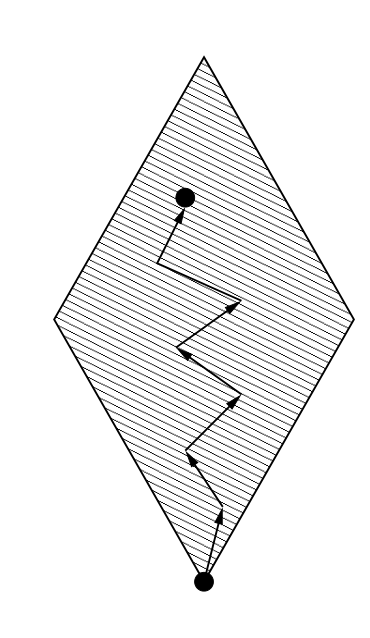
\includegraphics[width=\textwidth]{graphics/fixed-point_walk}
    \end{column}
  \end{columns}
\end{frame}

\begin{frame}{The Fixed Point Theorem}
  \begin{columns}[c]
    \begin{column}{0.8\textwidth}
      \noindent
      \[
      \begin{array}{l}
        \only<1>{\bot \sqsubseteq f(\bot) \phantom{\bot \sqsubseteq \dots}\\
        \phantom{}\\}
        \only<2->{\bot \sqsubseteq f(\bot) \sqsubseteq f^2(\bot) \sqsubseteq \dots\\
        \phantom{}\\}
        \onslide<3->{\dots \sqsubseteq f^k(\bot) =  f^{k+1}(\bot)\\
        \phantom{}\\}
        \onslide<4->{f^k(\bot) = fix(f)}
      \end{array}
      \]
    \end{column}

    \begin{column}<0->{0.2\textwidth}
      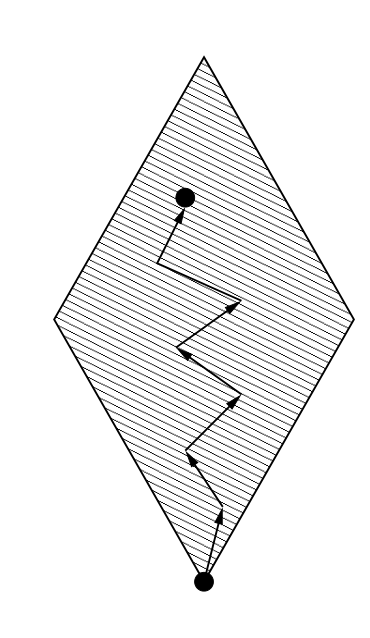
\includegraphics[width=\textwidth]{graphics/fixed-point_walk}
    \end{column}
  \end{columns}
\end{frame}


\begin{frame}{Constraint Rules}{}
  f is defined by constraint rules, applied on each CFG node:
  \[ F(x_1, \dots, x_n) = (F_1(x_1, \dots, x_n), \dots, F_n(x_1, \dots, x_n)) \]
\end{frame}


\begin{frame}{Constraint Rules}{Modified reaching definitions}
  Auxiliary function:
  \[ JOIN(v) = \bigcup_{ w \in pred(v)} \constraint{w} \]

  Non-assignment nodes:
    \[ \constraint{v} = JOIN(v) \]
\end{frame}


\begin{frame}{Constraint Rules}{Modified reaching definitions}
    Assignment nodes:
  \begin{align*}
  \constraint{v} = &\text{ if v is a reassignment:}\\
  &\phantom{==}JOIN(v) \cup \{ v \}\\
  &\text{ else:}\\
  &\phantom{==}JOIN(v) \downarrow id \cup \{ v \}\\
  \end{align*}
\end{frame}

\begin{frame}{Constraint Rules}
  Assignment nodes:
  \begin{align*}
  \constraint{v} = &\text{ if v is a reassignment:}\\
  &\phantom{==}JOIN(v) \cup \{ v \}\\
  &\text{ else:}\\
  &\phantom{==}JOIN(v) \downarrow id \cup \{ v \}\\
  \end{align*}
  \noindent\makebox[\linewidth]{\rule{\textwidth}{0.4pt}}
  \[
  \begin{array}{ll}
    v = source() &\\
    v = v + '!' & \phantom{ \{v = source(), v = v + '!'\}}\\ 
    v = \ 'harmless' & \\
    sink(v)& \\
  \end{array}
  \]
\end{frame}

\begin{frame}{Constraint Rules}
  Assignment nodes:
  \begin{align*}
  \constraint{v} = &\text{ if v is a reassignment:}\\
  &\phantom{==}JOIN(v) \cup \{ v \}\\
  &\text{ else:}\\
  &\phantom{==}JOIN(v) \downarrow id \cup \{ v \}\\
  \end{align*}
    \noindent\makebox[\linewidth]{\rule{\textwidth}{0.4pt}}
  \[
  \begin{array}{ll}
    v = source() & \{v = source()\}\\
    v = v + '!' &\phantom{ \{v = source(), v = v + '!'\}}\\
    v = \ 'harmless' & \\
    sink(v)& \\
  \end{array}
  \]
\end{frame}

\begin{frame}{Constraint Rules}
  Assignment nodes:
  \begin{align*}
  \constraint{v} = &\text{ if v is a reassignment:}\\
  &\phantom{==}JOIN(v) \cup \{ v \}\\
  &\text{ else:}\\
  &\phantom{==}JOIN(v) \downarrow id \cup \{ v \}\\
  \end{align*}
    \noindent\makebox[\linewidth]{\rule{\textwidth}{0.4pt}}
  \[
  \begin{array}{ll}
    v = source() & \{v = source()\}\\
    v = v + '!' & \{v = source(), v = v + '!'\}\\
    v = \ 'harmless' &\\
    sink(v)& \\
  \end{array}
  \]
\end{frame}

\begin{frame}{Constraint Rules}
  Assignment nodes:
  \begin{align*}
  \constraint{v} = &\text{ if v is a reassignment:}\\
  &\phantom{==}JOIN(v) \cup \{ v \}\\
  &\text{ else:}\\
  &\phantom{==}JOIN(v) \downarrow id \cup \{ v \}\\
  \end{align*}
    \noindent\makebox[\linewidth]{\rule{\textwidth}{0.4pt}}
  \[
  \begin{array}{ll}
    v = source() & \{v = source()\}\\
    v = v + '!' & \{v = source(), v = v + '!'\}\\
    v = \ 'harmless' & \{v = \ 'harmless'\}\\
    sink(v)& \\
  \end{array}
  \]
\end{frame}

\begin{frame}{Constraint Rules}
  Assignment nodes:
  \begin{align*}
  \constraint{v} = &\text{ if v is a reassignment:}\\
  &\phantom{==}JOIN(v) \cup \{ v \}\\
  &\text{ else:}\\
  &\phantom{==}JOIN(v) \downarrow id \cup \{ v \}\\
  \end{align*}
    \noindent\makebox[\linewidth]{\rule{\textwidth}{0.4pt}}
  \[
  \begin{array}{ll}
    v = source() & \{v = source()\}\\
    v = v + '!' & \{v = source(), v = v + '!'\}\\
    v = \ 'harmless' & \{v = \ 'harmless'\}\\
    sink(v)& \{v = \ 'harmless'\}\\
  \end{array}
  \]
\end{frame}


\begin{frame}{Lattice}
  \begin{tikzpicture}[remember picture,overlay]
    \fill [white] (current page.south west) rectangle (current page.north east);
    \node at (current page.center) {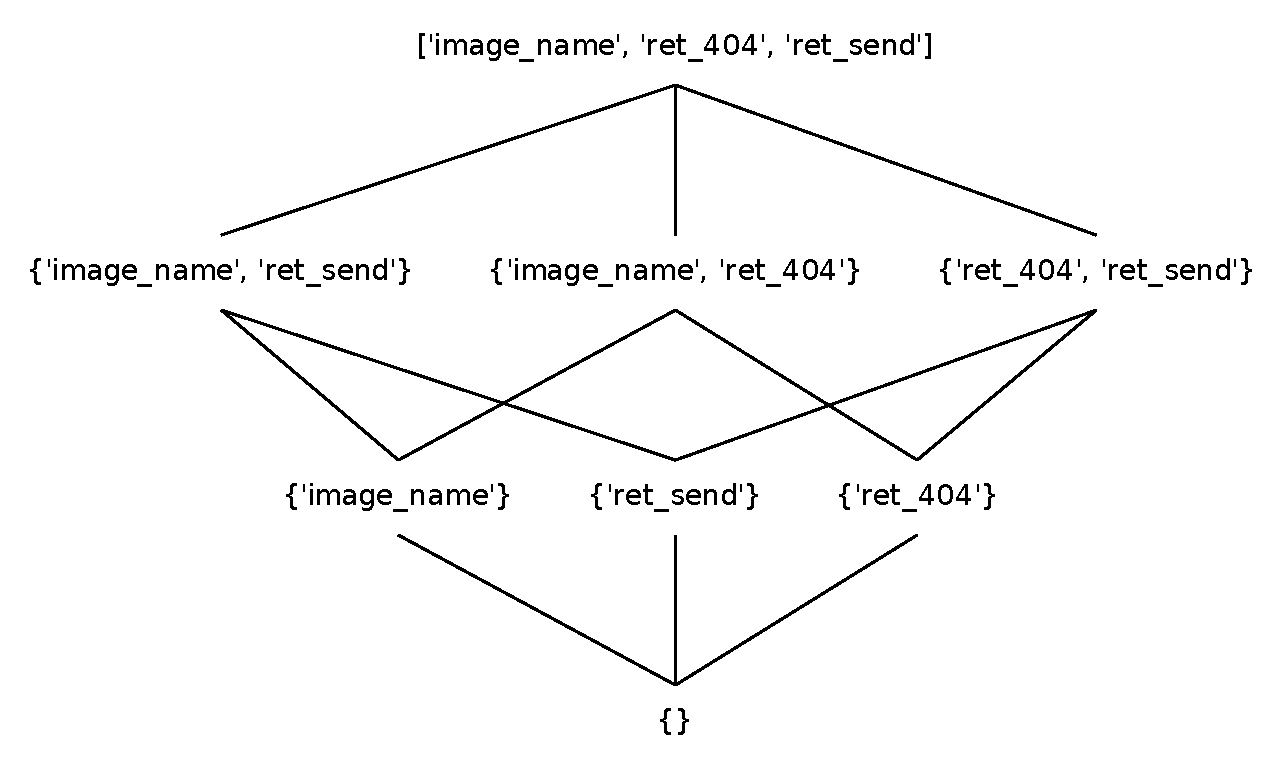
\includegraphics[width=1.1\textwidth]{graphics/path_traversal_lattice}};
    \end{tikzpicture}
  
\end{frame}


\begin{frame}{Fixed Point Iteration 1}
\[
\begin{array}{lclcl}
  \constraint{entry} & = & \{\} & &\\
  \assignconstraint{image} & = & \{\} &\\
  \constraint{if} & = & \{\}&\\
  \assignconstraint{ret\_404} & = & \{\}&\\
  \assignconstraint{ret\_send} & = & \{\}&\\
  \constraint{exit} & = & \{\}&\\
  && \phantom{\{command, paramssdd\}} && \phantom{\{command, param\}}
\end{array}
\]
\end{frame}

\begin{frame}{Fixed Point Iteration 1}
\[
\begin{array}{lclcl}
  \constraint{entry} & = & \{\} & \rightarrow & \{\}\\
  \assignconstraint{image} & = & \{\} & \rightarrow &\{image\}\\
  \constraint{if} & = & \{\} & \rightarrow &\{\}\\
  \assignconstraint{ret\_404} & = & \{\} & \rightarrow &\{ret\_404\}\\
  \assignconstraint{ret\_send} & = & \{\} & \rightarrow &\{ret\_send\}\\
  \constraint{exit} & = & \{\} & \rightarrow & \{\}\\
  && \phantom{\{command, param\}} && \phantom{\{command, param\}}
\end{array}
\]
\end{frame}

\begin{frame}{Fixed Point Iteration 2}
\[
\begin{array}{lclcl}
  \constraint{entry} & = & \{\} &&\\
  \assignconstraint{image} & = & \{image\} &&\\
  \constraint{if} & = & \{\} &&\\
  \assignconstraint{ret\_404} & = & \{ret\_404\} &&\\
  \assignconstraint{ret\_send} & = & \{ret\_send\} &&\\
  \constraint{exit} & = & \{\} &&\\
  && \phantom{\{command, param\}} && \phantom{\{command, param\}}
\end{array}
\]
\end{frame}

\begin{frame}{Fixed Point Iteration 2}
\[
\begin{array}{lclcl}
  \constraint{entry} & = & \{\} & \rightarrow & \{\}\\
  \assignconstraint{image} & = & \{image\} & \rightarrow &\{image\}\\
  \constraint{if} & = & \{\} & \rightarrow &\{image\}\\
  \assignconstraint{ret\_404} & = & \{ret\_404\} & \rightarrow &\{ret\_404\}\\
  \assignconstraint{ret\_send} & = & \{ret\_send\} & \rightarrow &\{ret\_send\}\\
  \constraint{exit} & = & \{\} & \rightarrow & \{ret\_send, ret\_404\}\\
  && \phantom{\{command, param\}} && \phantom{\{command, param\}}
\end{array}
\]
\end{frame}

\begin{frame}{Fixed Point Iteration 3}
\[
\begin{array}{lclcl}
  \constraint{entry} & = & \{\} &&\\
  \assignconstraint{image} & = & \{image\} &&\\
  \constraint{if} & = & \{image\} &&\\
  \assignconstraint{ret\_404} & = & \{ret\_404\} &&\\
  \assignconstraint{ret\_send} & = & \{ret\_send\} &&\\
  \constraint{exit} & = & \{ret\_send, ret\_404\} &&\\
  && \phantom{\{command, param\}} && \phantom{\{command, param\}}
\end{array}
\]
\end{frame}

\begin{frame}{Fixed Point Iteration 3}
\[
\begin{array}{lclcl}
  \constraint{entry} & = & \{\} & \rightarrow & \{\}\\
  \assignconstraint{image} & = & \{image\} & \rightarrow &\{image\}\\
  \constraint{if} & = & \{image\} & \rightarrow &\{image\}\\
  \assignconstraint{ret\_404} & = & \{ret\_404\} & \rightarrow &\{ret\_404, image\}\\
  \assignconstraint{ret\_send} & = & \{ret\_send\} & \rightarrow &\{ret\_send, image\}\\
  \constraint{exit} & = & \{ret\_send, ret\_404\} & \rightarrow & \{ret\_send, ret\_404\}\\
  && \phantom{\{command, param\}} && \phantom{\{command, param\}}
\end{array}
\]
\end{frame}


\begin{frame}{Fixed Point Iteration 4}
\[
\begin{array}{lclcl}
  \constraint{entry} & = & \{\} &&\\
  \assignconstraint{image} & = & \{image\} &&\\
  \constraint{if} & = & \{image\} &&\\
  \assignconstraint{ret\_404} & = & \{ret\_404, image\} &&\\
  \assignconstraint{ret\_send} & = & \{ret\_send, image\} &&\\
  \constraint{exit} & = & \{ret\_send, ret\_404\} &&\\
  && \phantom{\{command, param\}} && \phantom{\{command, param\}}
\end{array}
\]
\end{frame}

\begin{frame}{Fixed Point Iteration 4}
\[
\begin{array}{lclcl}
  \constraint{entry} & = & \{\} & \rightarrow & \{\}\\
  \assignconstraint{image} & = & \{image\} & \rightarrow &\{image\}\\
  \constraint{if} & = & \{image\} & \rightarrow &\{image\}\\
  \assignconstraint{ret\_404} & = & \{ret\_404\} & \rightarrow &\{ret\_404, image\}\\
  \assignconstraint{ret\_send} & = & \{ret\_send\} & \rightarrow &\{ret\_send, image\}\\
  \constraint{exit} & = & \{ret\_send, ret\_404\} & \rightarrow & \{ret\_send, ret\_404, image\}\\
  && \phantom{\{command, param\}} && \phantom{\{command, param\}}
\end{array}
\]
\end{frame}

\begin{frame}{Fixed Point Iteration 5}
\[
\begin{array}{lclcl}
  \constraint{entry} & = & \{\} &&\\
  \assignconstraint{image} & = & \{image\} &&\\
  \constraint{if} & = & \{image\} &&\\
  \assignconstraint{ret\_404} & = & \{ret\_404, image\} &&\\
  \assignconstraint{ret\_send} & = & \{ret\_send, image\} &&\\
  \constraint{exit} & = & \{ret\_send, ret\_404, image\} &&\\
  && \phantom{\{command, param\}} && \phantom{\{command, param\}}
\end{array}
\]
\end{frame}

\begin{frame}{Fixed Point Iteration 5}
\[
\begin{array}{lclcl}
  \constraint{entry} & = & \{\} & \rightarrow & \{\}\\
  \assignconstraint{image} & = & \{image\} & \rightarrow &\{image\}\\
  \constraint{if} & = & \{image\} & \rightarrow &\{image\}\\
  \assignconstraint{ret\_404} & = & \{ret\_404, image\} & \rightarrow &\{ret\_404, image\}\\
  \assignconstraint{ret\_send} & = & \{ret\_send, image\} & \rightarrow &\{ret\_send, image\}\\
  \constraint{exit} & = & \{ret\_send, ret\_404, image\} & \rightarrow & \{ret\_send, ret\_404,\\
&&&& \phantom{a}image\}
\end{array}
\]
\end{frame}

\begin{frame}{Flexible analysis}
  The analysis is flexible
  \begin{itemize}
    \item Can be exchanged
    \item Can be extended
  \end{itemize}

 Extension example:
  \begin{itemize}
    \item Dead code analysis
  \end{itemize}
  \center
  
\includegraphics[width=0.3\textwidth]{graphics/modular}
\end{frame}

